\documentclass[12pt,letterpaper]{article}
\usepackage{hyperref}
\hypersetup{colorlinks=true,allcolors=black}
\usepackage[utf8]{inputenc}
\usepackage[frenchb]{babel}
\usepackage[T1]{fontenc}
\usepackage{ae,aecompl}
\usepackage{pslatex}
\usepackage[top=2cm, bottom=2cm, left=2cm, right=2cm]{geometry}
\usepackage{hhline}
\usepackage{amsmath}
\usepackage{pgfplots}
\pgfplotsset{compat=newest}
\usepackage{multicol}
\usepackage{graphicx}
\graphicspath{{Images/}}
\hyphenpenalty=100
\usepackage{caption}
\usepackage{enumitem}
\usepackage{textcomp}
% Pour multicol (Align top)
\raggedcolumns
% Pour enlever l'indentation et avoir un espace entre les paragraphes
%\usepackage[parfill]{parskip}
\usepackage{float}
\floatstyle{plaintop}
\restylefloat{table}


\begin{document}
	
	%====== Page de presentation ======%
	\hypersetup{pageanchor=false}
	%================ Page titre ================

\title{
	\textbf{Plan de test} \\
	\vspace{2cm}
	Système de protection et de gestion de batterie Li-ion	
}
\author{
	Daigneault-St-Arnaud, Christian, DAIC30099006 \\
	Gagnon-Bourassa, Julien, GAGJ23108601 \\
	Cusson-Larocque, Olivier, CUSO09048905	
}
\newcommand{\cours}{ELE791 - Projets spéciaux }
\newcommand{\prof}{Deslandes, Dominic}



\makeatletter
\begin{titlepage}


	\pagenumbering{gobble}
	\centering
	{\Huge \@title}\\ 
	\vspace{3cm}
	{\large Par \\
		\vspace{0.5cm}
		\@author \\
		\vspace{3cm}
		\cours \\
		\vspace{0.5cm}
		\prof \\
		\vspace{3.5cm}
		\@date \\
		\vspace{3.5cm}
		\'{E}COLE DE TECHNOLOGIE SUP\'{E}RIEURE \\
		UNIVERSIT\'{E} DU QUÉBEC
	}
\end{titlepage}
\makeatother





	\newpage
	%====== Table des matieres ======%
	\pagenumbering{roman}
	\hypersetup{pageanchor=true}
	\tableofcontents
	%\listoftables
	%\listoffigures	
	%\newpage


%====================== INCLUSION DES PARTIES ======================
	\pagenumbering{arabic}
	
	%====== Objectif : Protection des modules ======%
	\section{Protection des modules}
	\paragraph*{}
	La protection des modules consiste à détecter une surcharge, une décharge excessive, un courant trop élevé et une température trop élevée. Suite à la détection d'une faute, le système de protection doit amener la batterie à un état sécuritaire indépendamment du conducteur. La réglementation exige que des indicateurs de fautes soient installés à l'extérieur du véhicule et sur le tableau de bord. La faute doit être verrouillée et cette dernière doit seulement être effacée manuellement lorsque le véhicule n'est pas en mouvement et que la faute n'est plus présente \cite{cahier_charge}.
	
	\paragraph*{}
	Pour détecter les différentes fautes, il est nécessaire d'avoir une lecture de la tension de chaque module, une lecture de la température des modules, une lecture du courant de la batterie et un algorithme de détection pour éviter de déclencher la protection pour un faux positif. Pour amener la batterie dans un état sécuritaire et indiquer qu'il y a une faute, le système doit avoir un bus de communication et un contrôle de l'état de la batterie très robuste. La ré-initialisation du système de protection requiert une interface accessible et un algorithme qui vérifie que les conditions sont adéquates. 
	


	
	%====== Fonctionnalité : Lecture de la tension des modules  ======%
	\subsection{Lecture de tension des modules}
	\paragraph*{}
	La majorité de l'information sur la batterie provient de la tension des modules, c'est pourquoi cette mesure doit être très précise et robuste sur toute la plage d'utilisation des modules. Le circuit doit consommer un minimum de courant, être robuste, modulable et précis. Le circuit doit aussi faciliter la vérification technique.
	
	\subsubsection*{Solution commerciale}
	\paragraph*{}
	Il existe sur le marché plusieurs circuits qui s'occupent de lire la tension des modules et de communiquer l'information à un microcontrôleur. Les fonctionnalités et le nombre de modules supportés varient d'un vendeur à l'autre. Les points communs sont : 

	\begin{multicols}{2}
		\begin{itemize}
			\item[$\bullet$] Le circuit peut être alimenté par les modules;
			\item[$\bullet$] Consommation de courant de quelque mA lorsque le circuit prend les mesures et quelques $\mu$A lorsqu'il est en veille;
			\item[$\bullet$] Solution compacte;
			\item[$\bullet$] Lecture précise;
			\item[$\bullet$] Les modules doivent être branchés dans l'ordre;
			\item[$\bullet$] Économique;
			\item[$\bullet$] Fonctionnement bien documenté.
		\end{itemize}
	\end{multicols}

	\paragraph*{}
	Cette solution est réalisable et demande surtout de bien lire et comprendre la documentation. Le LTC6804 de Linear Technology a été retenu pour son nombre de modules maximum, son prix et sa simplicité d'implémentation. Cette solution répond à la majorité des spécifications, mais elle n'apporte cependant rien de nouveau au système actuellement utilisé et elle ne facilite pas la vérification technique. 
	
	\newpage
	
	\subsubsection*{Isolation des lectures}
	\paragraph*{}
	La vérification technique sera beaucoup plus facile si les différentes lectures de tensions sont isolées. Ce point est décrit dans la section Facilité les manipulations lors des vérifications techniques. 
	
	\paragraph*{}
	L'isolation amène plusieurs avantages :
	
	\begin{itemize}
		\item[$\bullet$] Les modules n'ont plus besoin d'être branchés en ordre, ce qui élimine ce risque d'erreur humaine;
		\item[$\bullet$] Il est possible de débrancher une seule cellule pour venir ensuite la remplacer par une alimentation variable;
		\item[$\bullet$] Le filage dans la batterie peut être mieux organisé et optimisé.
	\end{itemize}

	\paragraph*{}
	Cette solution comporte cependant plusieurs désavantages :
	
	\begin{itemize}
		\item[$\bullet$] Consomme plus de courant (quelque mA par module lors des lectures);
		\item[$\bullet$] Demande plus de composantes;
		\item[$\bullet$] Plus difficile à implémenter;
		\item[$\bullet$] Plus dispendieux.
	\end{itemize}
	
	\paragraph*{}
	Ces différents désavantages ne sont pas majeurs dans le contexte d'Éclipse, la consommation de courant reste insignifiante comparée à ce que le moteur et le reste des circuits consomment. Le nombre de composants peut être limité en utilisant la bonne topologie et le prix de la carte peut être plus élevé tant qu'il respecte le budget. 
	
	\subsubsection*{Circuit analogique}
	\paragraph*{}
	Une solution relativement simple et qui ne comporte pas beaucoup de composantes est montrée à la figure \ref{fig:HCNR201}. Ce circuit très compact et simple n'est pas assez précis puisque le gain entre les deux photodiodes varie de 5\% pour le HCNR201. Cette erreur ne répond pas aux spécifications de +/- 10mV qui représente une erreur de $\pm 0.238 \%$ ($\pm 10mV / 4.2V \cdot 100 \%$).  
	
	\begin{figure}[H]
		\centering
		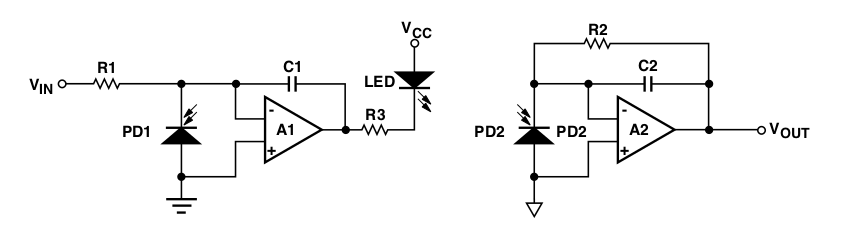
\includegraphics[scale = 0.5]{Images/Analogique.png}
		\caption{Circuit de lecture de tension isolé analogique \cite{HCNR201}}
		\label{fig:HCNR201}
	\end{figure}


	\newpage
	\subsubsection*{Lecture d'un voltage de référence avec un ADC}
	\paragraph*{}	
	Pour éliminer l'erreur causée par l'amplificateur et l'isolateur tout en réduisant au maximum le nombre de composants, l'ADC mesurerait un voltage de référence alors qu'il serait alimenté par le module comme présenté à la figure \ref{fig:adc_vref}. Puisque le voltage à l'entrée est connu, la tension du module est donnée par l'équation \ref{eq:vref}.
	
	\begin{align}
		V_{Module} = \dfrac{V_{REF}}{Valeur~ADC} \cdot 2^{~nb~Bits~adc}
		\label{eq:vref}
	\end{align}
	
	\begin{figure}[H]
		\centering
		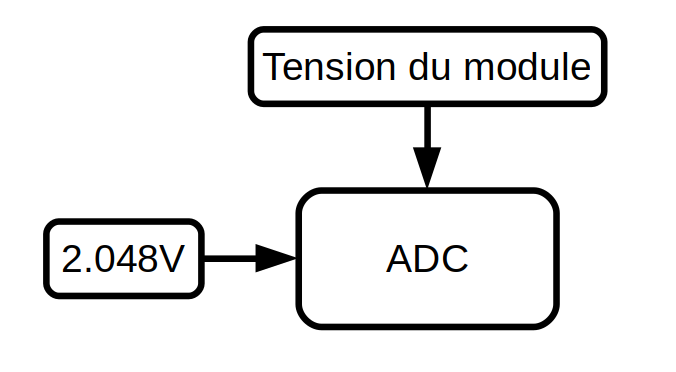
\includegraphics[scale=0.3]{Images/Voltage_reference.png}
		\caption{Lecture d'un voltage de référence avec un ADC}
		\label{fig:adc_vref}
	\end{figure}
	
	\paragraph*{}
	Le circuit mesure le LSB qui est donné par $V_{Module} / 2^{~nb~Bits~adc}$ pour  trouver la tension du module. Bien que cette technique fonctionne, les courbes de la tension du module et de la résolution ne sont pas linéaires par rapport au résultat du ADC. La valeur du voltage de référence à un impacte sur la courbe de la résolution. Plus il est bas, moins la courbe est linéaire et la résolution est moins bonne. Les figures \ref{fig:vmodule_vref} et \ref{fig:res_vref} montre les performances idéales du circuit à la figure \ref{fig:adc_vref} avec une référence de 2.048V et une plage de 2V à 4.2V pour la tension du module.
	
	\begin{figure}[H]
		\begin{minipage}{0.45\textwidth}
			\centering
			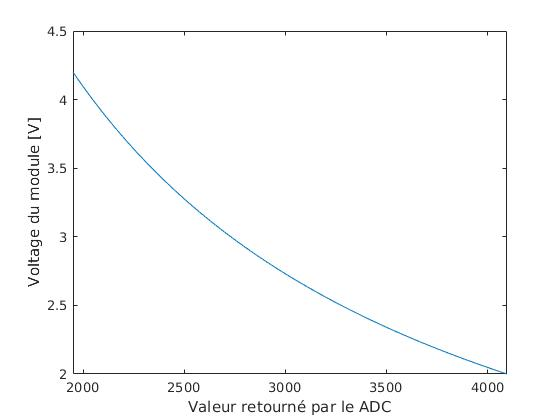
\includegraphics[scale=0.4]{Images/Vmodule_REF_2V.jpg}
			\caption{Tension du module en fonction des valeurs du ADC}
			\label{fig:vmodule_vref}
		\end{minipage}
		\hfill
		\begin{minipage}{0.45\textwidth}
			\centering
			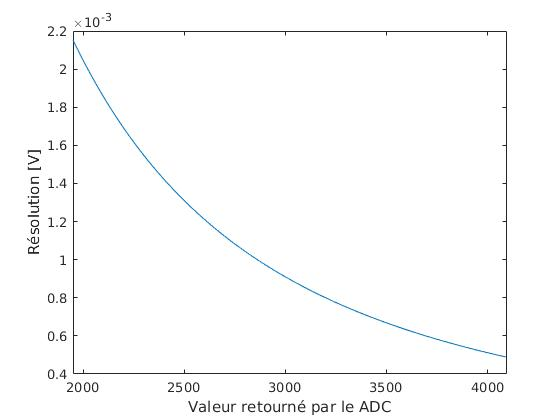
\includegraphics[scale=0.4]{Images/RES_REF_2V.jpg}
			\caption{Résolution en fonction des valeurs du ADC}
			\label{fig:res_vref}
		\end{minipage}	
	\end{figure}	
	
	\paragraph*{}
	L'écart maximal entre 2 bits est de 2.15 mA. Avec un ADC performant qui a une erreur de $\pm 1$ LSB, la lecture de tension à une erreur maximale de $\pm $ 2.15 mA lorsque le module est à 4.2V. Cette méthode correspond à la spécification qui demande d'être à $\pm $ 10 mA. L'ADC consomme et la tension de référence consomme très peu de courant, ils nécessitent très peu de composants externes et ils sont abordables. Afin d'avoir une très bonne précision, il est nécessaire de faire une calibration puisque la tolérance de la référence ($\pm$ 0.5 \%) est plus grande que celle de la spécification ($\pm 0.238 \%$). Il existe des références avec des tolérances plus petites que $\pm 0.238 \%$ mais elles sont beaucoup trop dispendieuses pour le projet puisqu'il faut en avoir une pour chaque module.    
	
	\paragraph*{}
	L'isolation de la mesure se fait au niveau de la communication puisqu'il n'y a aucune erreur causée par l'isolateur de cette façon, contrairement à l'optocoupleur de la solution analogique. L'alimentation de l'isolateur et du ADC doit dépasser la plage de lecture du module qui est de 2V à 4.5V.
	
	\paragraph*{}
	Cette solution est viable, elle respecte les spécifications et elle ne demande pas beaucoup de composantes. Le choix des ADC et des isolateurs numériques avec une alimentation qui va de moins de 2V à plus de 5V est toutefois très restreint. Les prix de l'isolateur et de l'ADC sont donc élevés et il est plus difficile de trouver un remplacement dans le cas ou un composant n'est plus disponible.   
	
	\subsubsection*{Configuration classique d'un ADC}
	\paragraph*{}
	Pour utiliser l'ADC avec une configuration classique où l'entrée mesure le voltage du module, un convertisseur de puissance est nécessaire pour maintenir une tension fixe qui est plus élevée que celle du module. Plusieurs composants externes sont nécessaires, mais les coûts sont absorbés par le prix moins élevé de l'ADC et de l'isolateur. Cette topologie permet d'avoir une résolution qui est fixe sur toute la plage des mesures, un contrôle sur le LSB avec l'alimentation de l'ADC et un meilleur choix d'ADC. Le ADC est alimenté par un régulateur linéaire pour avoir un minimum de bruit alors que l'isolateur est alimenté par le convertisseur à commutation. L'isolateur qui commute rapidement ne vient donc pas perturber l'alimentation de l'ADC. Puisque l'alimentation de l'ADC  est utilisée comme référence, il est important de faire une calibration pour avoir un LSB qui est très précis afin d'avoir une mesure qui respecte les spécifications. Avec la référence calibrée à 4.5V et un ADC qui à une erreur de $\pm$ 1 LSB, la précision de la mesure est de $\pm 1.1$ mV sur toute la plage. La tension du module est donnée par l'équation \ref{eq:Vmodule}.
	
	\begin{align}
		V_{Module} = \dfrac{V_{Ref}}{2^{~nb~Bits~adc}} \cdot \text{Valeur ADC}
		\label{eq:Vmodule}
	\end{align}
	
	\begin{figure}[H]
		\centering
		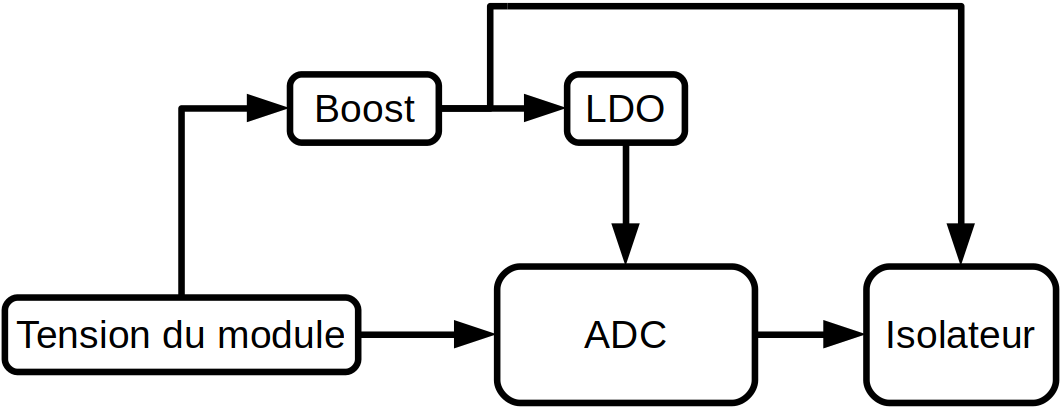
\includegraphics[scale=0.3]{Images/Tension_module.png}
		\caption{Lecture de la tension du module}
		\label{fig:adc_vmod}
	\end{figure}	

	\paragraph*{}
	Le nombre de composants rend cette solution plus dure à implémenter en raison de l'espace restreint que les modules esclaves peuvent prendre dans la batterie. Les composants devront être choisis en fonction de leurs performances et leur format. Cette topologie offre de bonnes performances et elle n'est pas plus dispendieuse que la solution précédente. 
	
	\subsubsection*{Choix final}
	\paragraph*{}	
	La topologie utilisée pour mesurer la tension des modules sera la configuration classique. Ses performances malgré sa complexité en font le meilleur choix puisqu'il sera impossible de faire une deuxième version de la carte avant la fin du projet. L'option la plus sécuritaire, éprouvé et qui permet un grand choix de pièce est plus avantageuse que la première option qui n'est pas assez précise et la deuxième qui nécessite des composantes avec des caractéristiques très restreintes. La solution commerciale a été écartée puisqu'il serait beaucoup plus dur d'incorporer des sécurités pour les mauvaises manipulations et faciliter la vérification technique.	
	%====== Fonctionnalité : Lecture de du courant  ======%
	
\subsection{Contrôle des contacteurs}

	\paragraph*{}
	Pour amener la batterie dans un état sécuritaire, il faut pouvoir la débrancher de l'alimentation. Le système utilise donc des contacteurs à haute puissance pour contrôler la connexion de la batterie avec le reste des charges. 
	
	\paragraph*{}
	Le module maître se charge de contrôler ces contacteurs. Il s'occupe de connecter les batteries lors de la mise en marche du système ou de les déconnecter en cas de défaillances pour protéger les modules.

	\paragraph*{}
	Le système est composé de trois contacteurs, soient deux contacteurs principaux et un pour les MPPTs. L'un des contacteurs principaux est connecté à la borne positive de la batterie et l'autre à la borne négative. On peut voir à la figure suivante un schéma général de la disposition des contacteurs. 
	
	\begin{figure}[H]
		\centering
		\fbox{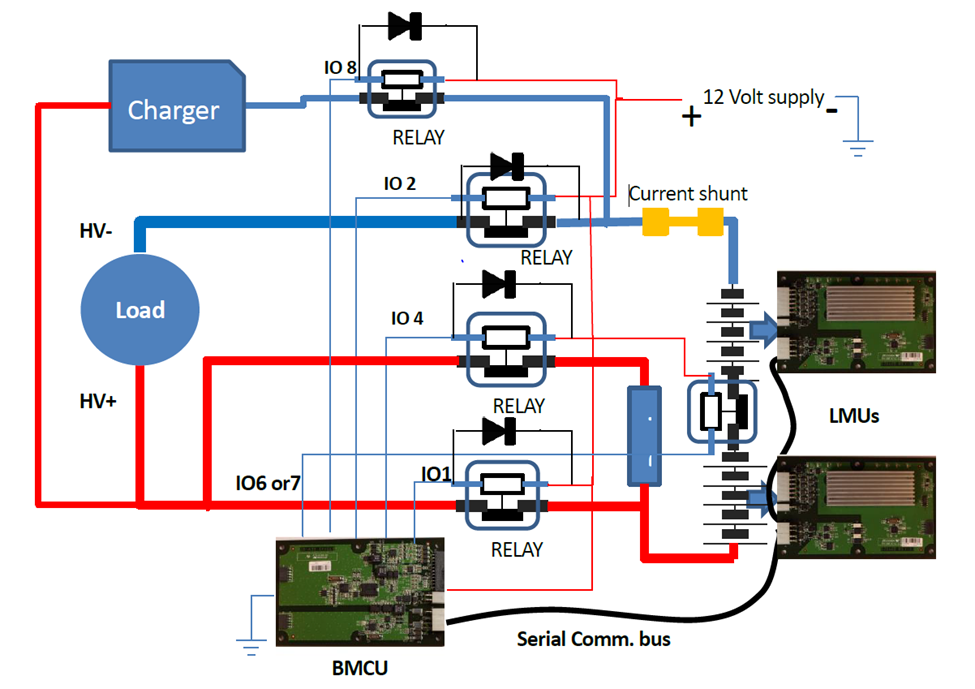
\includegraphics[width=0.6\linewidth]{Images/LithiumBalanceContactorDiagram}}
		\caption{Diagramme général des contacteurs de LithiumBalance \cite{Lithium_Balance}}
		\label{fig:lithiumbalancecontactordiagram}
	\end{figure}

	\paragraph*{}
	L'enclenchement des contacteurs se fait avec une tension de 12V, qui doit être appliquée à ses bornes. Puisque c'est le microcontrôleur qui envoie la commande d'ouverture ou de fermeture, il doit y avoir une interface de protection entre le 12V aux bornes du contacteur et le 3.3V de la patte GPIO. De façon générale, il n'est pas conseillé d'utiliser des actionneurs mécaniques, tel qu'un relais, pour activer les contacteurs puisqu'ils sont souvent victimes de défaille. 	 

	\subsubsection*{Choix des contacteurs:}
		\paragraph*{}
		Une commandite d'Autobus Lion a permis au club Éclipse de se procurer trois contacteurs de marque GIGAVAC\_HX21. Il faut donc que le module maître puisse interfacer ces contacteurs. Le système de batterie d'Éclipse 9 utilise des contacteurs EV200 et ceux-ci seront utilisés comme pièce de remplacement. La conception du circuit de contrôle doit donc être compatible avec les deux modèles.

		\paragraph*{}
		Les spécifications des contacteurs Gigavac montrent que le courant consommé lors de l'ouverture de l'inductance est de 4.3 A. En ajoutant une marge de protection d'un facteur de 1.2, les composantes doivent soutenir un courant allant jusqu'à 5.16 A pendant 75 ms\cite{GigavacHX21}. 

		\paragraph*{}
		De plus, ce modèle de contacteur possède un deuxième relais interne pour de l'interverrouillage (interlock), beaucoup utilisé dans le domaine des véhicules. Dans le cas du présent système, ce relais sera utilisé pour activer un témoin lumineux afin d'avertir l'utilisateur de l'état des contacteurs. Avec les contacteurs EV-200, il faudra court-circuiter deux positions sur le connecteur allant sur le module maître pour activer le témoin lumineux.

		\paragraph*{}
		Également, le circuit de contrôle doit répondre aux critères suivants afin d'être jugé sécuritaire \cite{System_Approach}.

		\begin{itemize}
			\item Prévenir les défaillances qui causent les contacteurs à ouvrir alors qu'ils devraient être fermés
			\item Prévenir les défaillances qui causent les contacteurs à fermer alors qu'ils devraient être ouverts
			\item Prévenir les défaillances qui causent une connexion de la batteries à travers une charge capacitive	
		\end{itemize}


	\subsubsection*{Choix du circuit de contrôle}
		\paragraph*{}
		Plusieurs solutions ont été évaluées pour contrôler les contacteurs. Parce que cette section est très critique et qu'il ne faut absolument pas qu'une défaillance met en panne la voiture solaire durant la compétition. C'est pourquoi le budget n'est pas un critère de sélection mais, plutôt le choix doit se faire sur une solution qui est le plus sécuritaire possible.

		\paragraph*{Solution 1: Contrôle par optocoupleurs}
		\paragraph*{}			
		Puisque les activateurs ne doivent pas être de nature mécanique. On peut utiliser des optocoupleurs (Solid State Relays) puisqu'ils sont isolés mécaniquement. Le microcontrôleur doit seulement activer une DEL de l'optocoupleur pour l'enclencher. Aussi, dans l'éventualité où le microcontrôleur ait une défaillance, l'optocoupleur s'ouvrira, empêchant ainsi le contacteur de rester fermé. Il faut par contre choisir un optocoupleur capable d'accepter jusqu'à 5.16 A, ce qui limite beaucoup le choix des composantes.
		
		\begin{table}[H]
			\centering
			\caption{Comparaison des optocoupleurs}
			\label{ComparaisonOpto}
			\renewcommand{\arraystretch}{1.3}
			\begin{tabular}{|p{3cm}|p{3cm}|p{3cm}|p{3cm}|}
				\hline
				\textbf{Optocoupleurs} & \textbf{Courant} & \textbf{Résistance} & \textbf{Prix}
				\\ \hhline{|=|=|=|=|}
				CPC1907B & 6 A & 60 mOhm & 9.01 \$ \\ \hline
				CPC1709J & 10 A & 50 mOhm & 10.00 \$ \\ \hline
				CPC1918J & 5.25 A &	100 mOhm & 14.83 \$	\\ \hline
			\end{tabular}
		\end{table}
		
		Le prix de ces composantes est similaire et leur courant de charge est assez robuste. Le choix s'est donc faite sur le CPC17907B en raison de son profil plat qui était plus avantageux avec le placement des pièces sur le module maître.
		
		\begin{figure}[H]
			\centering
			\fbox{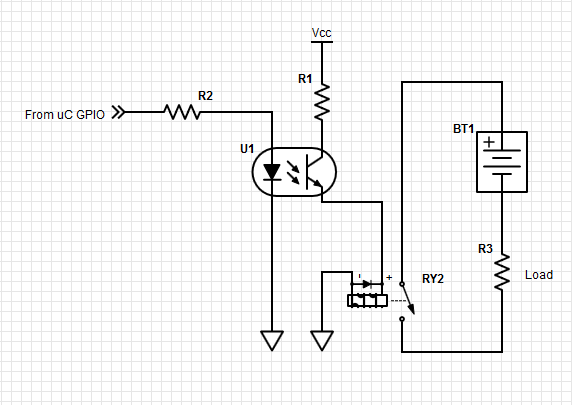
\includegraphics[width=0.4\linewidth]{../Images/ContactorSol1}}
			\caption[]{Schéma Solution 1: Contrôle par optocoupleurs}
			\label{fig:contactorsol1}
		\end{figure}
		
		
		\paragraph*{Solution 2: Contrôle par Mosfet en série}
		\paragraph*{}
		Une façon d'assurer la protection d'un circuit est de rajouter de la redondance. Plusieurs Mosfets sont mises en série pour augmenter les chances d'ouverture de circuit en cas de défaillances. Plus il y a de composantes en série, meilleures sont les chances, mais on augmente aussi le prix des composantes. Chaque Mosfet doit être contrôlé individuellement par une patte du microcontrôleur. Également, il est important de s'assurer que la résistance interne des Mosfets soit constante d'une composante à l'autre. Cela évite l'échauffement du Mosfet ayant la résistance interne la plus élevée, pouvant causer des défaillances.
		
		\begin{figure}[H]
			\centering
			\fbox{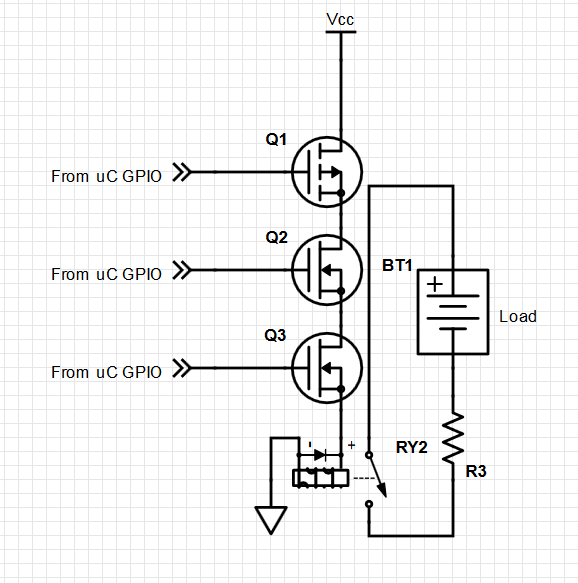
\includegraphics[width=0.4\linewidth]{../Images/ContactorSol2}}
			\caption{Schéma Solution 2: Contrôle par Mosfet en série}
			\label{fig:contactorsol2}
		\end{figure}
		

		\paragraph*{Solution 3: Circuit d'alimentation à double actionneurs}
		\paragraph*{}
		Cette solution provient du livre "A systems approach to Lithium-Ion Battery Management" \cite{System_Approach}. L'auteur propose d'utiliser circuit d'alimentation à doubles actionneurs, soit un actionneur sur le pôle négatif et un sur le pôle positif. Un Mosfet de type-P alimente le côté positif (High-side) et un mosfet de type-N est relié au commun sur le circuit du côté négatif (low-side) ce qui offre une sécurité supplémentaire si une des deux composantes venait à faillir. Puisqu'il y a trois contacteurs dans le système, cette solution requiert d'utiliser un seul Mosfet type-P pour alimenter le côté positif des contacteurs et trois Mosfets type-N pour le côté négatif de chaque relais.

		\begin{figure}[H]
			\centering
			\fbox{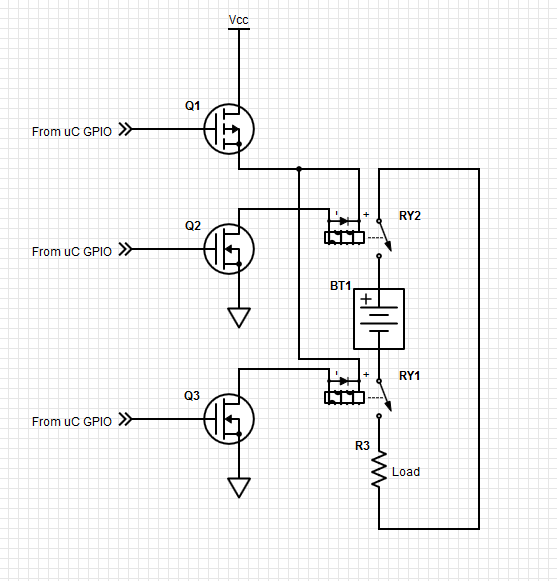
\includegraphics[width=0.4\linewidth]{../Images/ContactorSol3}}
			\caption{Schéma solution 3: Circuit d'alimentation à doubles actionneurs}
			\label{fig:contactorsol3}
		\end{figure}
		
		\paragraph*{Choix final}
		\paragraph*{}
		La solution retenue est un mélange de la solution 1 et 3. En ayant un circuit d'alimentation à doubles actionneurs, on évite d'avoir de la redondance. On remplace ainsi les mosfets de cette solution par les optpocoupleurs de la solution 1. De cette façon, on s'assure de la plus haute protection tout en ayant le minimum de composantes. Puis, puisqu'on veut éviter de tirer trop de courant du microcontrôleur, on utilise un transistor BJT s'activant avec un faible courant. Le BJT peut ensuite alimenter l'optocoupleur avec l'alimentation 3.3V directement.

		\begin{figure}[H]
			\centering
			\fbox{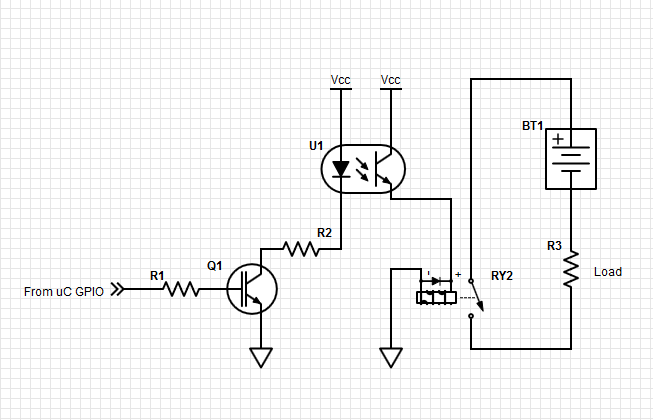
\includegraphics[width=0.4\linewidth]{../Images/ContactorSolFinal}}
			\caption{Choix final}
			\label{fig:contactorsolfinal}
		\end{figure}

	\subsubsection*{Circuit de précharge:}
		\paragraph*{}
		Le contacteur du MPPT et le contacteur principal sur le pôle positif de la batterie possèdent un circuit de précharge. La précharge permet à la batterie de se connecter à une large charge capacitive. Si la batterie est connectée directement avec une charge capacitive déchargée, le courant transitoire sera limité par l'impédance interne de la batterie, de la charge et des contacteurs. Cette limite ne sera généralement pas assez pour prévenir un courant potentiellement dangereux. Un contacteur qui s'enclenche lorsque la différence de potentiel est trop élevée pourrait le souder et empêcher son ouverture\cite{System_Approach}.
		
		\paragraph*{}
		Pour prévenir ce problème, on ajoute une résistance en série avec un relais, installés en parallèle du contacteur. Avant d'enclencher le contacteur, un courant limité passe par la résistance, et permet à la tension de monter de façon exponentielle. On compare ensuite la lecture de la charge avec la tension des batteries. Lorsque la tension sur la charge est assez élevée et que la différence de potentiel aux bornes du contacteur est négligeable, le contacteur peut être fermé de façon sécuritaire\cite{System_Approach}.
		
		\paragraph*{}		
		La résistance de précharge est dimensionnée pour dissiper la puissance circulant dans la résistance. Pour trouver cette valeur, il faut d'abord calculer la constante de temps\cite{LiIonBms}.
	
		\begin{align}
			\tau =R \cdot C
			\label{eq:Constante de temps}
		\end{align}
				
		On considère la charge capacitive complète après	
	 
		\begin{align}
			T = 5 \cdot \tau
			\label{eq:CapaciteCharge}
		\end{align}
		
		Par mesure de sécurité, on ajoute 0.5 seconde à ce chiffre.
		
		\begin{align}
			T = T + 0.5
			\label{eq:Tempsdecharge}
		\end{align}		
				
		On calcul ensuite l'énergie dissipée par la résistance de précharge.
		
		\begin{align}
			E = \dfrac{C \cdot V^2}{2}
			\label{eq:EnergiePrecharge}
		\end{align}
		
		On trouve finalement la puissance totale consommée par la résistance de précharge
	
		\begin{align}
			P = \dfrac{E}{T}
			\label{eq:PuissancePrecharge}
		\end{align}	
			
		\paragraph*{}		
		Le temps de précharge doit être judicieusement choisi pour s'assurer que la charge capacitive est assez chargée. D'après ces calculs, avec une résistance de 100 Ohm, une durée de 5.5 secondes sera nécessaire si l'on estime la charge capacitive est de 10000uF avec une tension maximale de 160V. On devrait dissiper environ 23.3 W durant cette période. Cependant, des tests devront être effectuer durant la réalisation pour ajuster ces valeurs.
				
		\begin{table}[H]
			\centering
			\caption{Sélection de la résistances de précharge}
			\label{ResistancePrecharge}
			\renewcommand{\arraystretch}{1.3}
			\begin{tabular}{|p{3cm}|p{5cm}|p{2cm}|p{2cm}|p{1.5cm}|}
				\hline
				\textbf{Composante} & \textbf{Manufacturier} & \textbf{Resistance} & \textbf{Pdissipation} & \textbf{Prix}
				\\ \hhline{|=|=|=|=|=|}
				TR50JBC100R & Stackpole Electronics Inc. & 100 Ohm & 50 W & 5.81 \$ \\ \hline		
			\end{tabular}
		\end{table}

		\paragraph*{}		
		Le relais doit supporter un courant de 1.6 A. Sa bobine devrait également consommer le moins possible. Un relais tout usage à été choisi.
		
		\begin{table}[H]
			\centering
			\caption{Sélection du relais}
			\label{RelaisPrecharge}
			\renewcommand{\arraystretch}{1.3}
			\begin{tabular}{|p{3cm}|p{3cm}|p{3cm}|p{3cm}|p{3cm}|}
				\hline
				\textbf{Composante} & \textbf{Manufacturier} &  \textbf{Courant} & \textbf{Consommation} & \textbf{Prix}
				\\ \hhline{|=|=|=|=|=|}
				ALQ312 & Panasonic & 10A & 16.7 mA & 3.34 \$ \\ \hline		
			\end{tabular}
		\end{table}				
		
	
		\paragraph*{}	
		Pour éviter de polariser à l'inverse les contacteurs avec la précharge, une diode est ajoutée au circuit. Elle doit bloquer une tension minimum de 160 V et pouvoir supporter un courant d'au moins 1.6 A. 
		
		\begin{table}[H]
			\centering
			\caption{Sélection de la diode}
			\label{DiodePrecharge}
			\renewcommand{\arraystretch}{1.3}
			\begin{tabular}{|p{3cm}|p{3cm}|p{3cm}|p{3cm}|p{3cm}|p{3cm}|}
				\hline
				\textbf{Composante} & \textbf{Manufacturier} & \textbf{Courant} &  \textbf{Baisse de tension} & \textbf{Prix}
				\\ \hhline{|=|=|=|=|=|=|}
				NRVBS3200T3G & ON Semiconductor & 3A & 840 mV @ 3A & 1.37 \$ \\ \hline		
			\end{tabular}
		\end{table}				
		
		\paragraph*{}			
		Ensuite, pour éviter qu'un courant trop élevé ne vienne endommager les composantes, on ajoute un fusible de 2A à action retardée. 
		
		\paragraph*{}			
		La topologie générale du circuit de précharge est présenté à la figure \ref{fig:circuitprecharge}.
				
		\begin{figure}[H]
			\centering
			\fbox{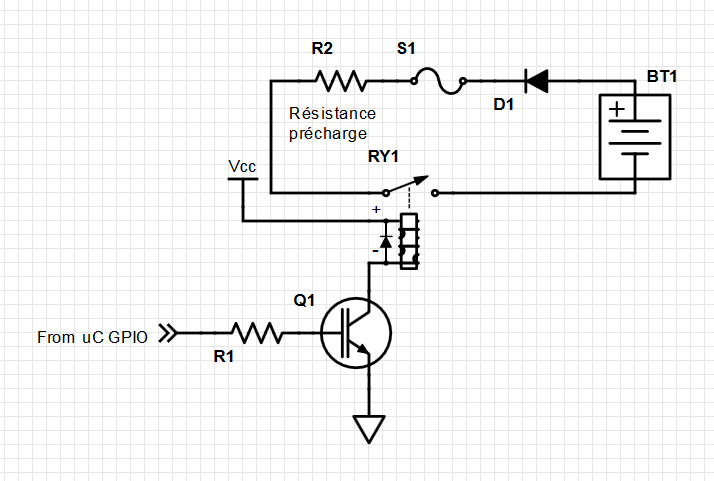
\includegraphics[width=0.7\linewidth]{Images/CircuitPrecharge}}
			\caption[]{Schéma du circuit de précharge}
			\label{fig:circuitprecharge}
		\end{figure}
			
		

	%====== Fonctionnalité : Lecture de la température  ======%
	
	%====== Fonctionnalité : Détection des seuils et sécurisation de la batterie  ======%

	%====== Fonctionnalité : Avertir l'utilisateur  ======%
	
\subsection{Avertie l'utilisateur}

	\paragraph*{}
	Message CAN vers board des lumières pour alumière externe
	LED driver erreur externe pour cockpit
	Led d'erreur sur le master board
		
	%====== Fonctionnalité : Réinitialisation  ======%
	\subsection{Réinitialisation du système}

\paragraph*{}
Message d'erreur Message CAN

LED driver erreur externe
Led d'erreur sur le master board
	
	%====== Objectif : Balancement des modules ======%
	

	%====== Objectif : Compatibilité avec le BMS présentement utilisé ======%
	
	
	%====== Objectif : Facilité les manipulations lors des vérifications techniques ======%

	%====== Architecture ======%
	\section{Architecture}
	
	\subsection{Architecture générale}
		\begin{figure}[H]
			\centering
			\fbox{\includegraphics[width=0.7\linewidth]{"Images/Architecture_generale"}}
			\caption{Architecture générale du système de protection et de contrôle}
			\label{fig:architecture_generale}
		\end{figure}
	
	\subsection{Architecture du module de lecture de courant}
		\begin{figure}[H]
			\centering
			\fbox{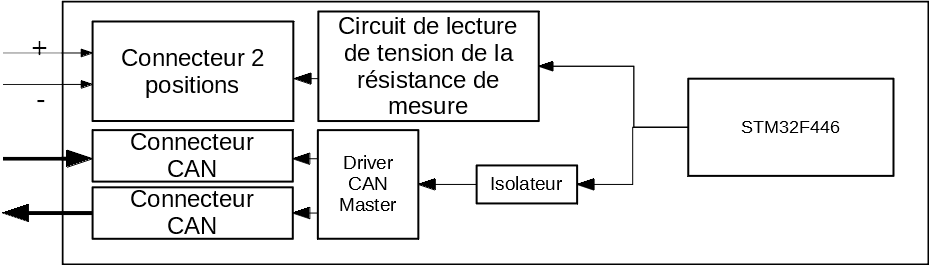
\includegraphics[width=0.7\linewidth]{Images/Architecture_LectureCourant}}
			\caption{Architecture du module de lecture de courant}
			\label{fig:architecturelecturecourant}
		\end{figure}
	\subsection{Architecture du module maître}
	
		\begin{figure}[H]
			\centering
			\fbox{\includegraphics[width=0.7\linewidth]{"Images/Architecture_Master"}}
			\caption{Architecture du module maître}
			\label{fig:architecture_master}
		\end{figure}

	\subsection{Architecture du module esclave}
	
	\begin{figure}[H]
		\centering
		\fbox{\includegraphics[width=0.7\linewidth]{"Images/Architecture_Slave"}}
		\caption{Architecture du module esclave}
		\label{fig:architecture_slave}
	\end{figure}


	
	\subsection{Choix technologiques}
	\subsubsection*{Système d'exploitation en temps réel}
		\paragraph*{}
		Le système d’exploitation en temps réel (RTOS) est utilisé pour rendre le système plus robuste. Il permet de facilement prioriser les tâches les plus importantes du système ainsi que d’améliorer son déterminisme. De plus, il rend la modification et la maintenance du code très simple grâce à la segmentation de l’application en tâches distinctes. Plusieurs RTOS sont disponibles et offrent des caractéristiques similaires. Les grands différenciateurs sont le coût, la robustesse (évaluée selon son utilisation dans des systèmes critiques), la licence utilisée pour le code et la facilité d’utilisation.

		\begin{table}[H]
			\centering
			\caption{Comparaison des RTOS}
			\label{my-label}
			\renewcommand{\arraystretch}{1.3}
			\begin{tabular}{|p{2cm}|p{2cm}|p{4cm}|p{3cm}|p{4cm}|}
				\hline &
				\textbf{Prix} & \textbf{Robustesse} & \textbf{Licence} & \textbf{Facilité}
				\\ \hhline{|=|=|=|=|=|}
				uC/OS-III &
				Gratuit (pour les étudiants et hobbyistes) &
				Certifié aérospatial, médical et industriel.
				Utilisé dans le « rover » Curiosity de la NASA. &
				Propriétaire mais à sources ouvertes. &
				Plateforme de développement déjà construite et prête à être utilisée.
				Connu des membres de l’équipe.
				Documentation exceptionnelle.
				\\ \hline
				FreeRTOS &
				Gratuit &
				Aucune certification. Pour avoir une version certifiée, il faut utiliser une version payante (SafeRTOS). &
				FreeRTOS Open Source License (GNU GPL modifiée). &
				Projet de base facilement générable à l’aide d’outils.
				Bonne documentation.
				\\ \hline
				RTEMS &
				Gratuit &
				Aucune information sur les certifications disponible.
				Utilisé dans l’espace par la NASA et l’ESA. &
				RTEMS License (GNU GPL modifiée). &
				Complexe.
				Bonne documentation.                                                                              \\ \hline
			\end{tabular}
		\end{table}

		\paragraph*{}
		Notre choix s’est arrêté sur uC/OS-III, surtout à cause de la facilité d’utilisation étant donné qu’une plateforme était déjà disponible et utilisée dans le club Éclipse. Le fait de réutiliser cette même plateforme nous fait gagner du temps et permettra à d’autres membres du club de pouvoir facilement intégrer le projet et l’améliorer au fil du temps. La robustesse du RTOS était aussi un point majeur, puisque le BMS est une application critique pour la vie.

	\subsubsection*{Protocole de communication}
		\paragraph*{}
		Nous avions le choix d’interfacer les périphériques externes avec plusieurs protocoles de communication. Les deux plus populaires sont le I2C et le SPI. Le I2C nécessite seulement deux traces pour relier tous les périphériques externes avec le microcontrôleur aux dépens d’une plus grande complexité dans la façon de communiquer. Quant au SPI, c’est le contraire. La façon de l’utiliser est très simple, mais il faut trois traces plus une supplémentaire pour chaque périphérique externe. De plus, le SPI peut aller a des vitesses plus grandes que le I2C.

		\paragraph*{}
		Notre choix s’est arrêté sur le SPI à cause de sa simplicité d’utilisation. Plus le code pour le gérer est simple, plus il est facile à tester et donc plus il a de chance d’être parfaitement robuste rapidement. Le microcontrôleur choisi peut accommoder le nombre de traces supplémentaires nécessaires, ce qui n’entraîne donc aucun coût supplémentaire relié au désavantage du SPI par rapport au I2C.

	\subsubsection*{Interruption et interrogation (polling)}
		\paragraph*{}
		Nous avons décidé de minimiser l’utilisation des interruptions à ce qui est vraiment nécessaire étant donné que lorsqu’une interruption est déclenchée, le système priorise le traitement de celle-ci par rapport au reste des fonctions. Les interruptions sont utiles pour obtenir un temps de réponse très rapide pour les fonctions prioritaires et de la précision pour les bases de temps (time base). Par contre, dépendamment des situations, elles peuvent ajouter une charge non négligeable sur le système et pourraient faire en sorte de le bloquer complètement s’il y avait une erreur de programmation dans les fonctions qui les prennent en charge. Si l’interruption est externe, comme pour un bouton, il est aussi dangereux qu’elle soit déclenchée sans le vouloir à cause d’un « glitch ».

	\subsubsection*{Microcontrôleur}
		\paragraph*{}
		Une multitude de marques de microcontrôleur existent sur le marché. Une des plus populaires est STMicroeletronics avec sa gamme STM32. Celle-ci est basée sur l’architecture la plus répandue pour le développement embarqué, soit l’ARM Cortex-M.

		\paragraph*{}
		Le choix de cette gamme repose sur plusieurs facteurs distinctifs. Premièrement, des cartes d’évaluation sont offertes à très faible coût, ce qui permet de commencer le développement avant d’avoir reçu le vrai matériel. Ensuite, une suite logicielle permettant d’utiliser les périphériques internes très facilement est disponible. De plus, une plateforme utilisant cette gamme de microcontrôleurs est déjà utilisée par le club scientifique Éclipse. Il y a donc déjà des connaissances acquises quant à son utilisation.

	\subsection{Logiciel}
	\paragraph*{}
	L'architecture logicielle des trois modules est présentée ici sous forme de pile montrant ainsi les interdépendances entre chaque couche. La première couche est pour l'applicatif. On y trouve les différentes tâches que le module doit effectuer. Ensuite viennent la couche des "middlewares", puis celle des services. Les services sont des librairies logicielles contextualisées qui utilisent les pilotes pour effectuer des tâches de plus haut niveau. Les trois dernières couches sont celles des pilotes, de l'abstraction matérielle et des périphériques matériels internes.

	\newpage
	\subsubsection*{Module maître}
		\noindent
		Interruptions : Base de temps du HAL, base de temps du RTOS, CAN \#1 (Tx et Rx),  CAN \#2 (Tx et Rx) \\
		Interrogations : ADC interne thermistor (x1), Bouton de reprise d’erreur
		\begin{figure}[H]
			\centering
			\fbox{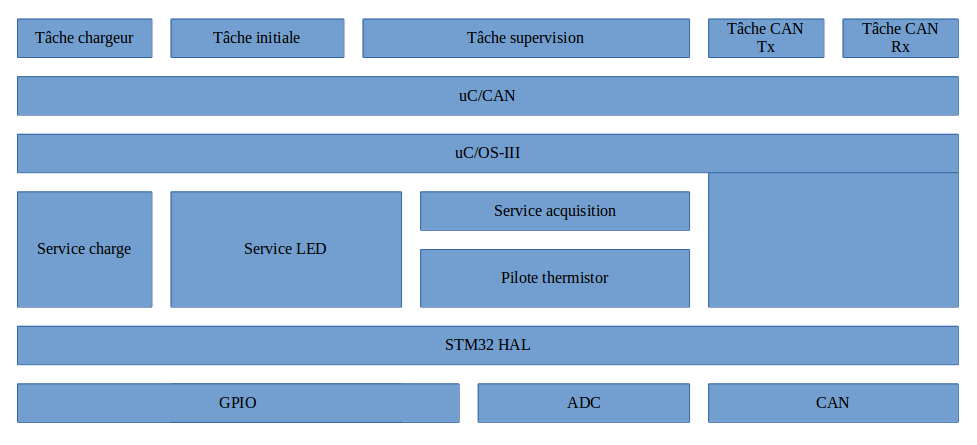
\includegraphics[scale=0.5]{Images/Logiciel_Master.png}}
			\caption{Logiciel du module maître}
			\label{fig:logiciel_master}
		\end{figure}
	
	\subsubsection*{Module esclave}
		\noindent
		Interruptions : Base de temps du HAL, base de temps du RTOS, CAN \#1 (Tx et Rx) \\
		Interrogations : ADC externe cellules (x8), ADC interne thermistor (x2)
		\begin{figure}[H]
			\centering
			\fbox{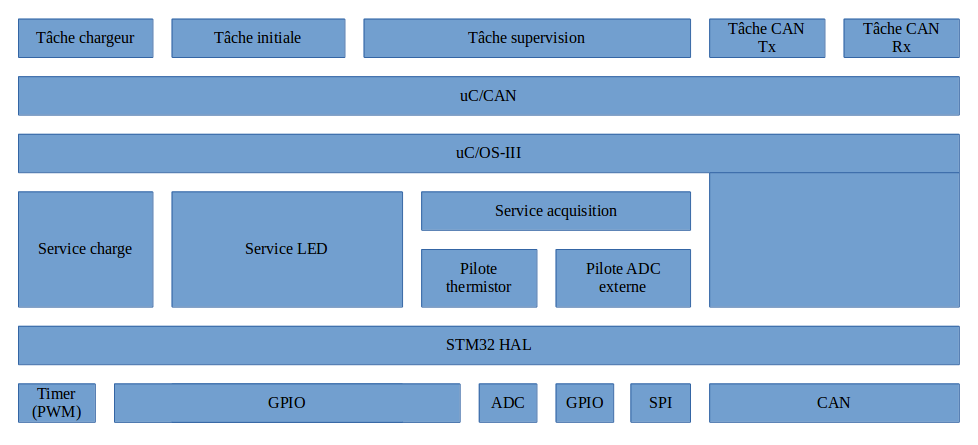
\includegraphics[scale=0.5]{Images/Logiciel_Slave.png}}
			\caption{Logiciel du module esclave}
			\label{fig:logiciel_slave}
		\end{figure}
	
	\newpage
	\subsubsection*{Module de lecture de courant}
		\noindent
		Interruptions : Base de temps du HAL, base de temps du RTOS, CAN \#1 (Tx et Rx) \\
		Interrogations : ADC externe shunt
		\begin{figure}[H]
			\centering
			\fbox{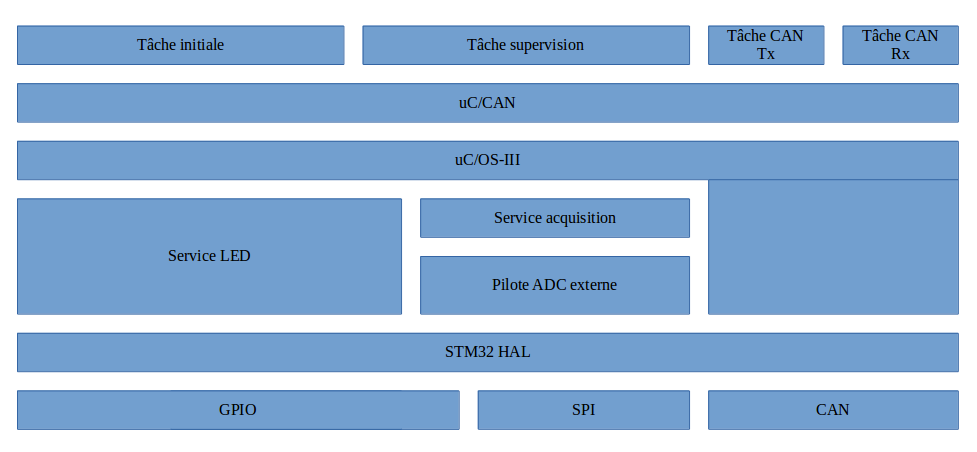
\includegraphics[scale=0.5]{Images/Logiciel_Current_Sense.png}}
			\caption{Logiciel du module de lecture de courant}
			\label{fig:logiciel_current_sense}
		\end{figure}

	\section{Diagrammes fonctionnels}
	\paragraph*{}
	\subsection{Module maître}
		\paragraph*{}
		
		\begin{figure}[H]
			\centering
			\fbox{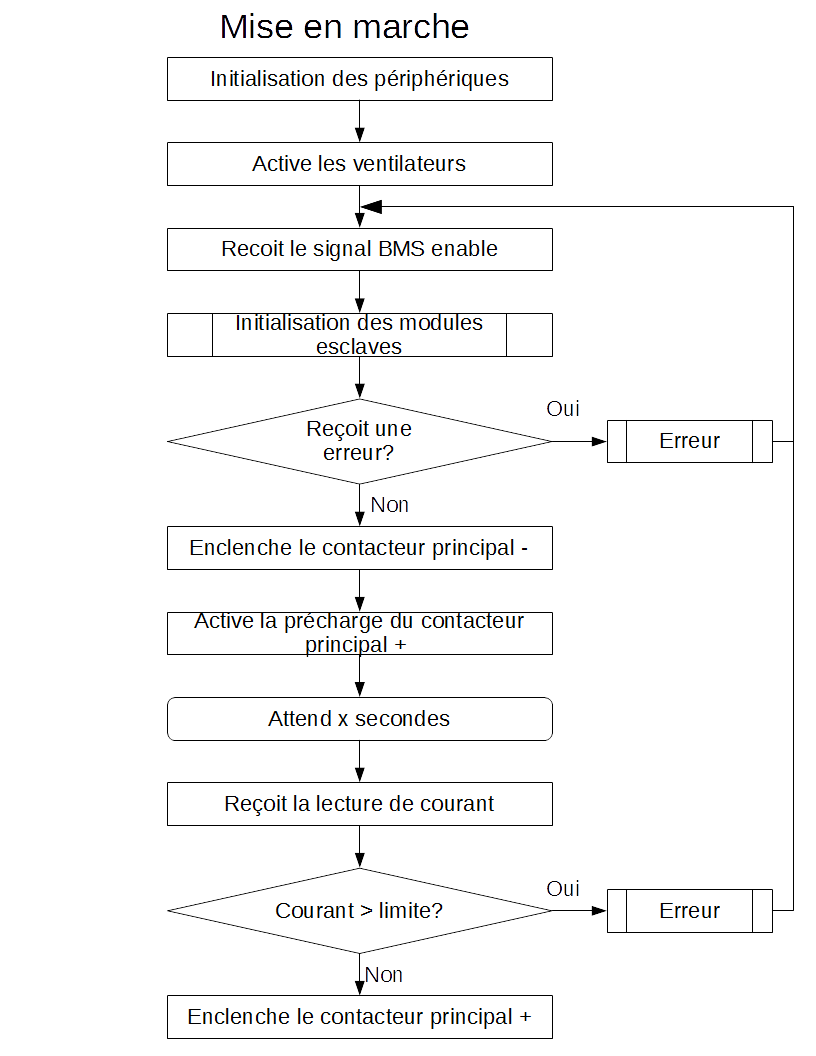
\includegraphics[width=0.5\linewidth]{Images/DiagrammeFonctionnel_MiseEnMarche}}
			\caption{Diagramme module maître: Mise en marche}
			\label{fig:diagrammefonctionnelmiseenmarche}
		\end{figure}
		
		\begin{figure}[H]
			\centering
			\fbox{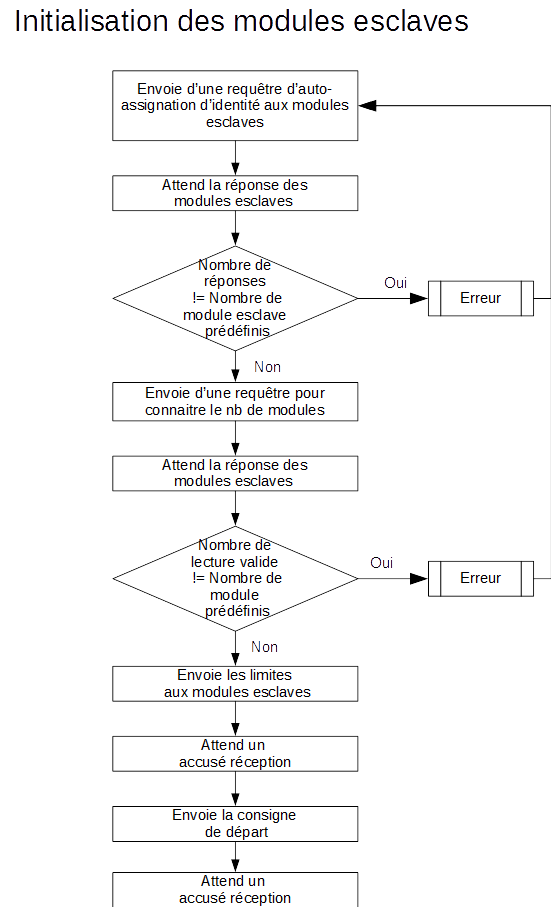
\includegraphics[width=0.7\linewidth]{Images/DiagrammeFonctionnel_MaitreInitEsclave}}
			\caption{Diagramme module maître: Initialisation des modules esclaves}
			\label{fig:diagrammefonctionnelmaitreinitesclave}
		\end{figure}
		
		\begin{figure}[H]
			\centering
			\fbox{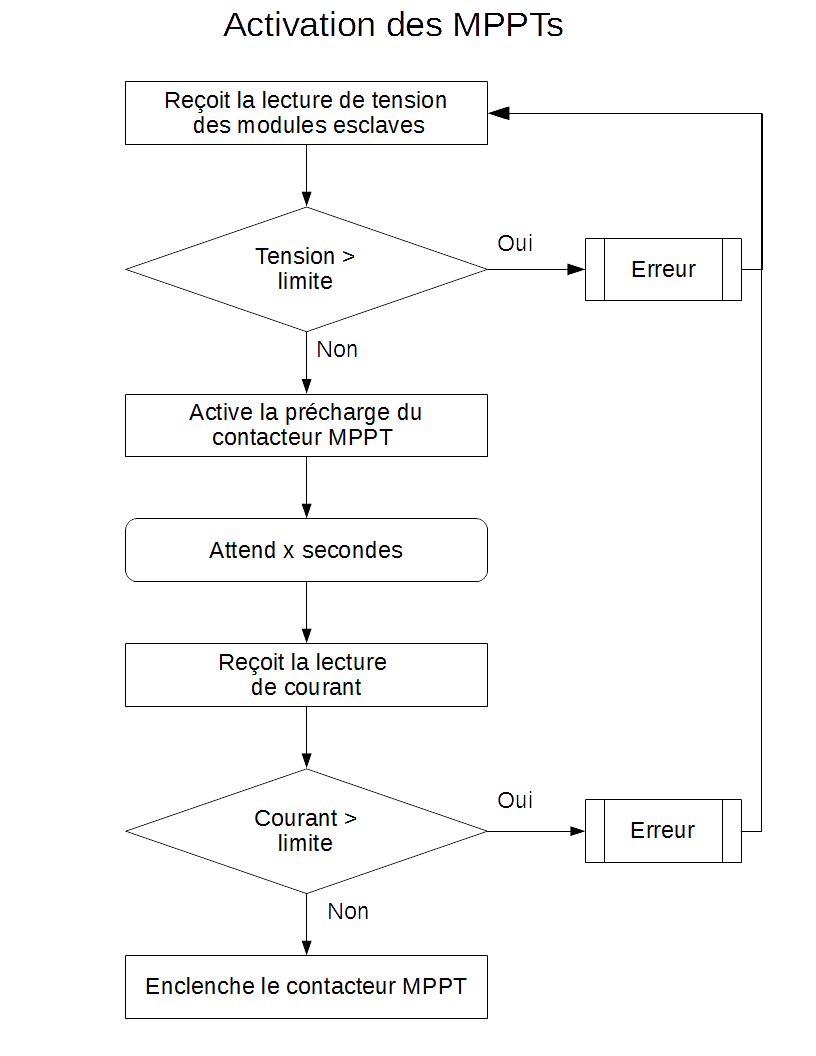
\includegraphics[width=0.7\linewidth]{Images/DiagrammeFonctionnel_ActivationMppt}}
			\caption{Diagramme module maître: Activation des MPPTs}
			\label{fig:diagrammefonctionnelactivationmppt}
		\end{figure}
		
		\begin{figure}[H]
			\centering
			\fbox{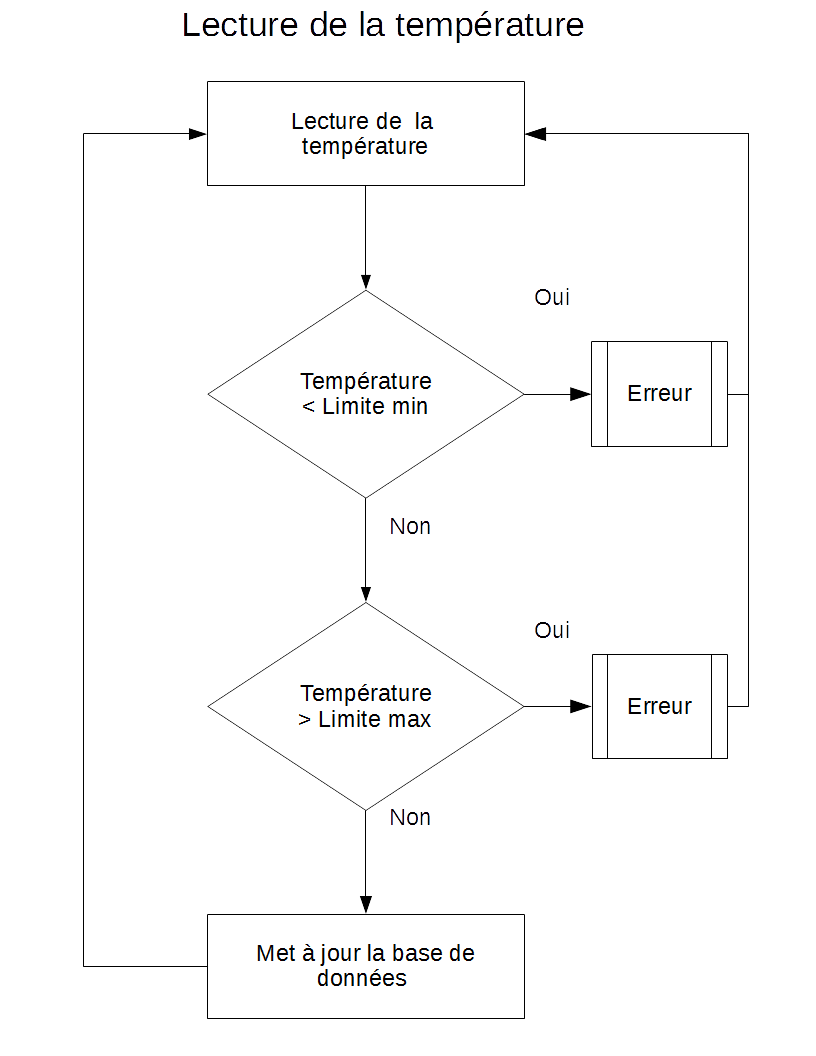
\includegraphics[width=0.7\linewidth]{Images/DiagrammeFonctionnel_MaitreLectureTemp}}
			\caption{Diagramme module maître: Lecture de la température}
			\label{fig:diagrammefonctionnelmaitrelecturetemp}
		\end{figure}
			
		\begin{figure}[H]
			\centering
			\fbox{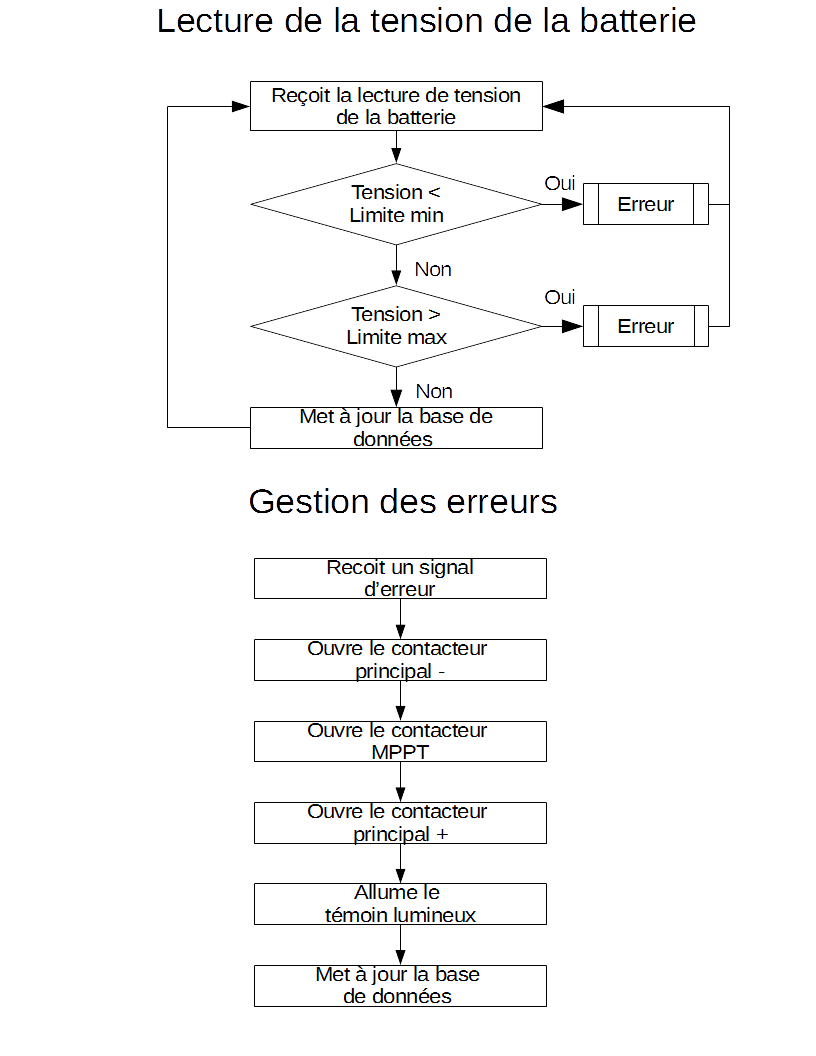
\includegraphics[width=0.7\linewidth]{Images/DiagrammeFonctionnel_MaitreLectureBat}}
			\caption{Diagramme module maître: Lecture de la tension de la batterie + Gestion des erreurs}
			\label{fig:diagrammefonctionnelmaitrelecturebat}
		\end{figure}
			
		\begin{figure}[H]
			\centering
			\fbox{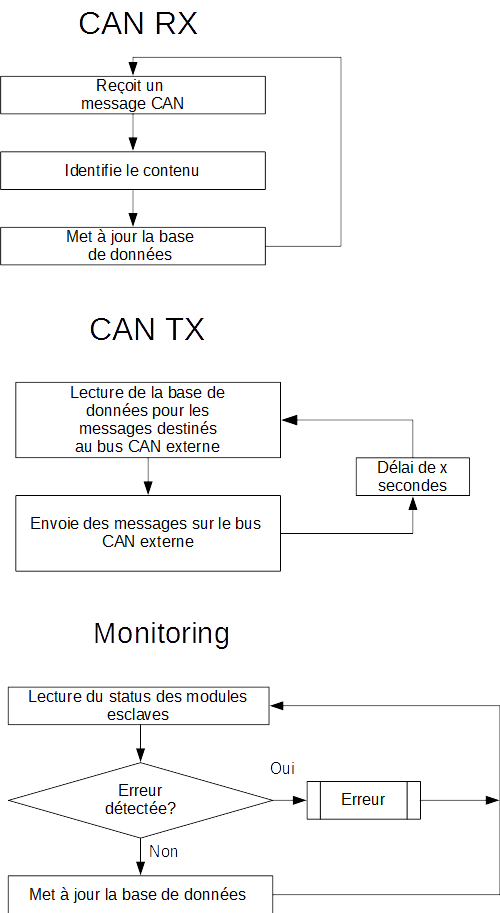
\includegraphics[width=0.7\linewidth]{Images/DiagrammeFonctionnel_CanMonitoring}}
			\caption{Diagramme module maître: CAN RX + CAN TX + Monitoring }
			\label{fig:diagrammefonctionnelcanmonitoring}
		\end{figure}
		
		
	\subsection{Module esclave}
		\paragraph*{}
	\subsection{Module de lecture de courant}
		\paragraph*{}


%====================== Bibliographie ======================

	\begin{thebibliography}{10}
	
	\bibitem{cahier_charge} 
	Christian Daigneault-St-Arnaud, Julien Gagnon-Bourassa, Olivier Cusson-Larocque. \textit{Cahier des charges, Système de protection et de gestion de batterie Li-ion}. \par	
	
	\bibitem{HCNR201} 
	Avago Technologies. \textit{HCNR200 and HCNR201 Data Sheet}.\\ \texttt{\url{https://docs.broadcom.com/docs/AV02-0886EN}}\par

	\bibitem{HCNR201} 
	Avago Technologies. \textit{HCNR200 and HCNR201 Data Sheet}.\\ \texttt{\url{https://docs.broadcom.com/docs/AV02-0886EN}}\par	
	
	
	\end{thebibliography}	
	
\end{document}



